
\DIFaddbegin 

\clearpage
\subsection{\DIFadd{The Weaver merchant}}
\label{sec:appendix:moj:weaver}

\DIFadd{A Viking weaver is called a vefari. Clothes were very valuable in the Viking Age because they took so long to make. It would take hours just to produce the raw fibres.
}

\begin{display}{The weaver stall}
	\label{fig:appendix:moj:places:weaver:stall}
	\DIFadd{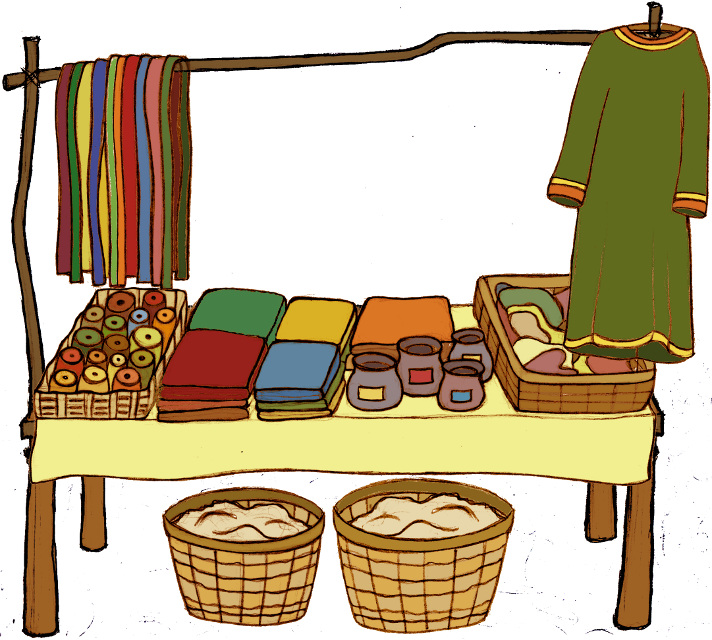
\includegraphics[width=0.65\columnwidth]{img/Jorvik/places/weaver stall}
}\end{display}

\begin{display}{The weaver stall with a background and a merchant}
	\label{fig:appendix:moj:places:weaver}
	\DIFadd{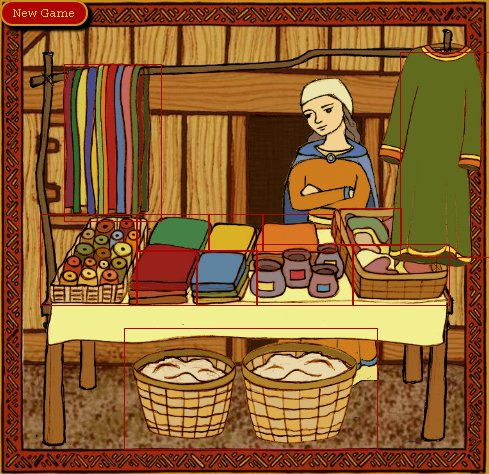
\includegraphics[width=0.65\columnwidth]{img/Jorvik/places/weaver}
}\end{display}
\clearpage


\begin{table}[ht!]
	\centering
	\begin{tabular}{ p{3cm} c }\toprule
		\textbf{\DIFaddFL{Name:}} & \multirow{5}{*}{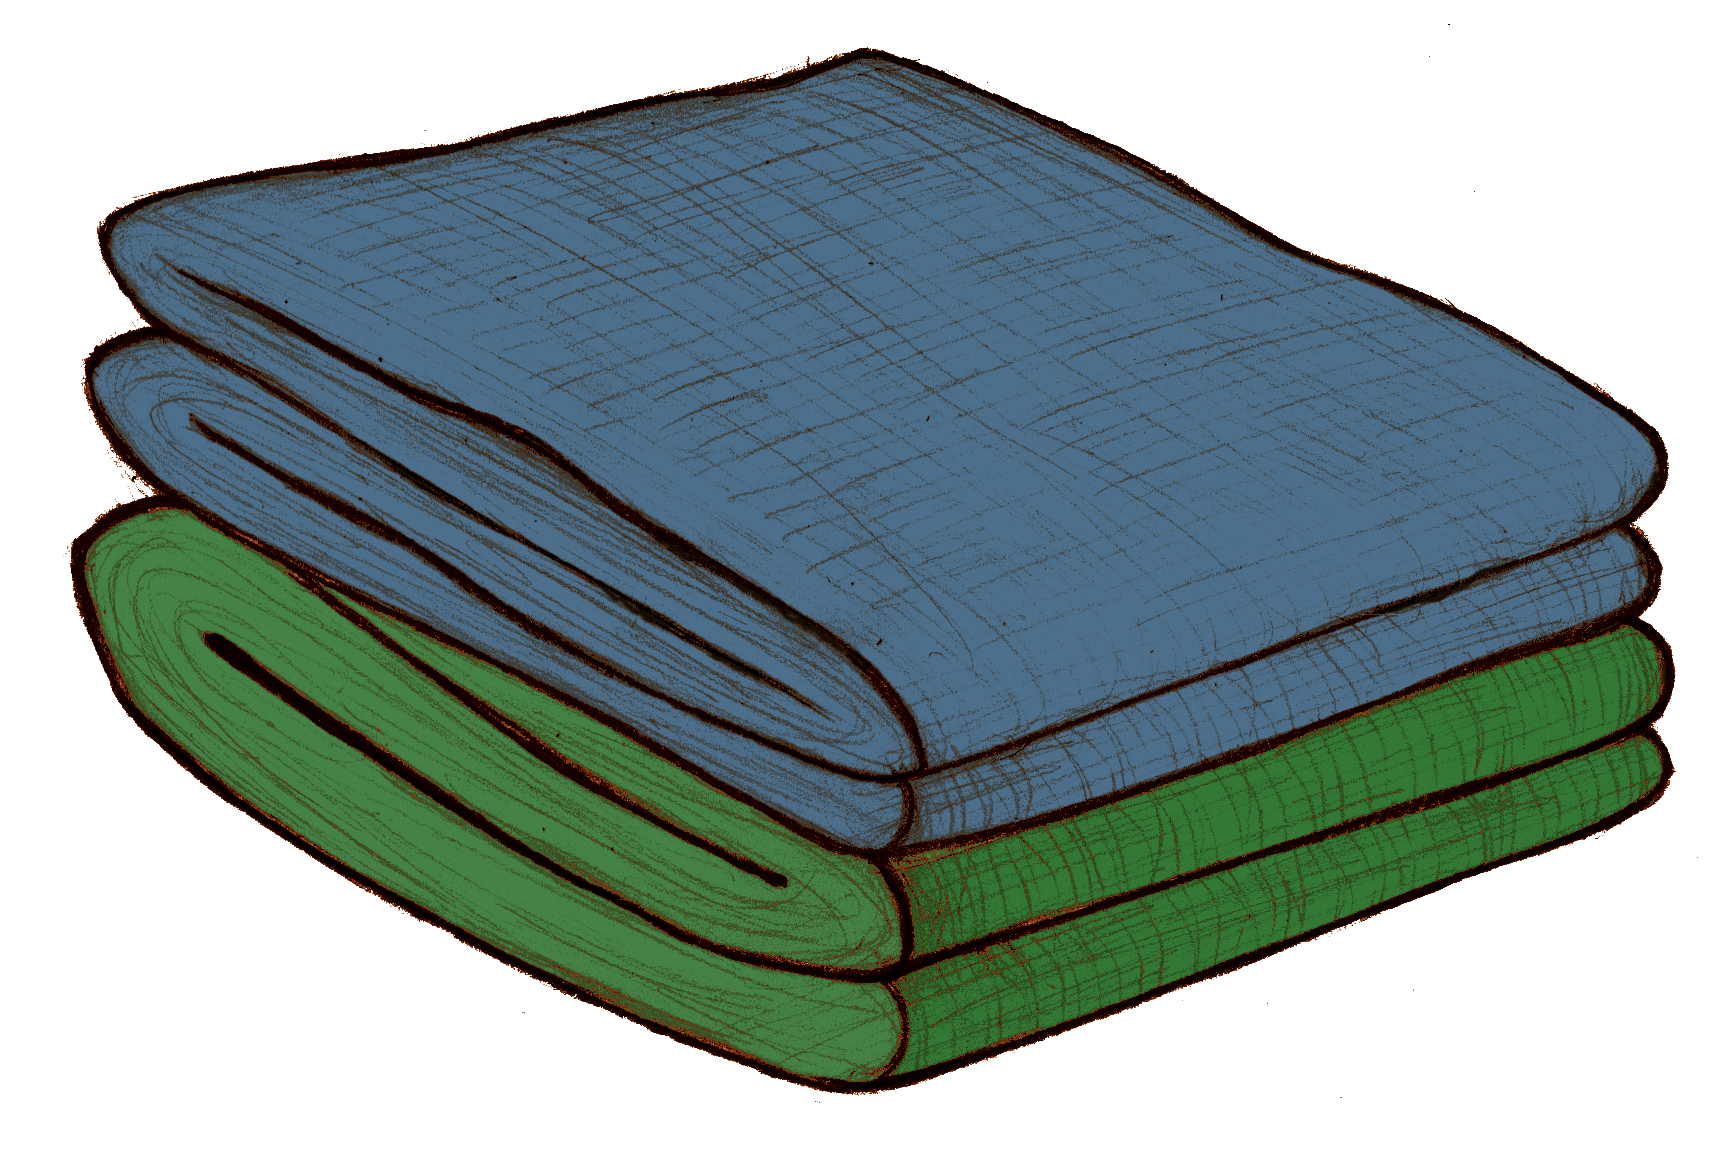
\includegraphics[height=30mm]{img/Jorvik/objects/weaver/cloth}}\\
		\DIFaddFL{Cloth }& \\ 
		\textbf{\DIFaddFL{Price:}} & \\
		\DIFaddFL{4.41  Silver. }& \\ 
		\textbf{\DIFaddFL{Description:}} & \\
		\multicolumn{2}{p{12cm}}{The Vikings in Iceland exported homespun cloth. Homespun cloth was used as a standard exchange product like the silver coins that were used across the world.}\\
		\bottomrule
	\end{tabular}
\end{table}

\begin{table}[ht!]
	\centering
	\begin{tabular}{ p{3cm} c }\toprule
		\textbf{\DIFaddFL{Name:}} & \multirow{5}{*}{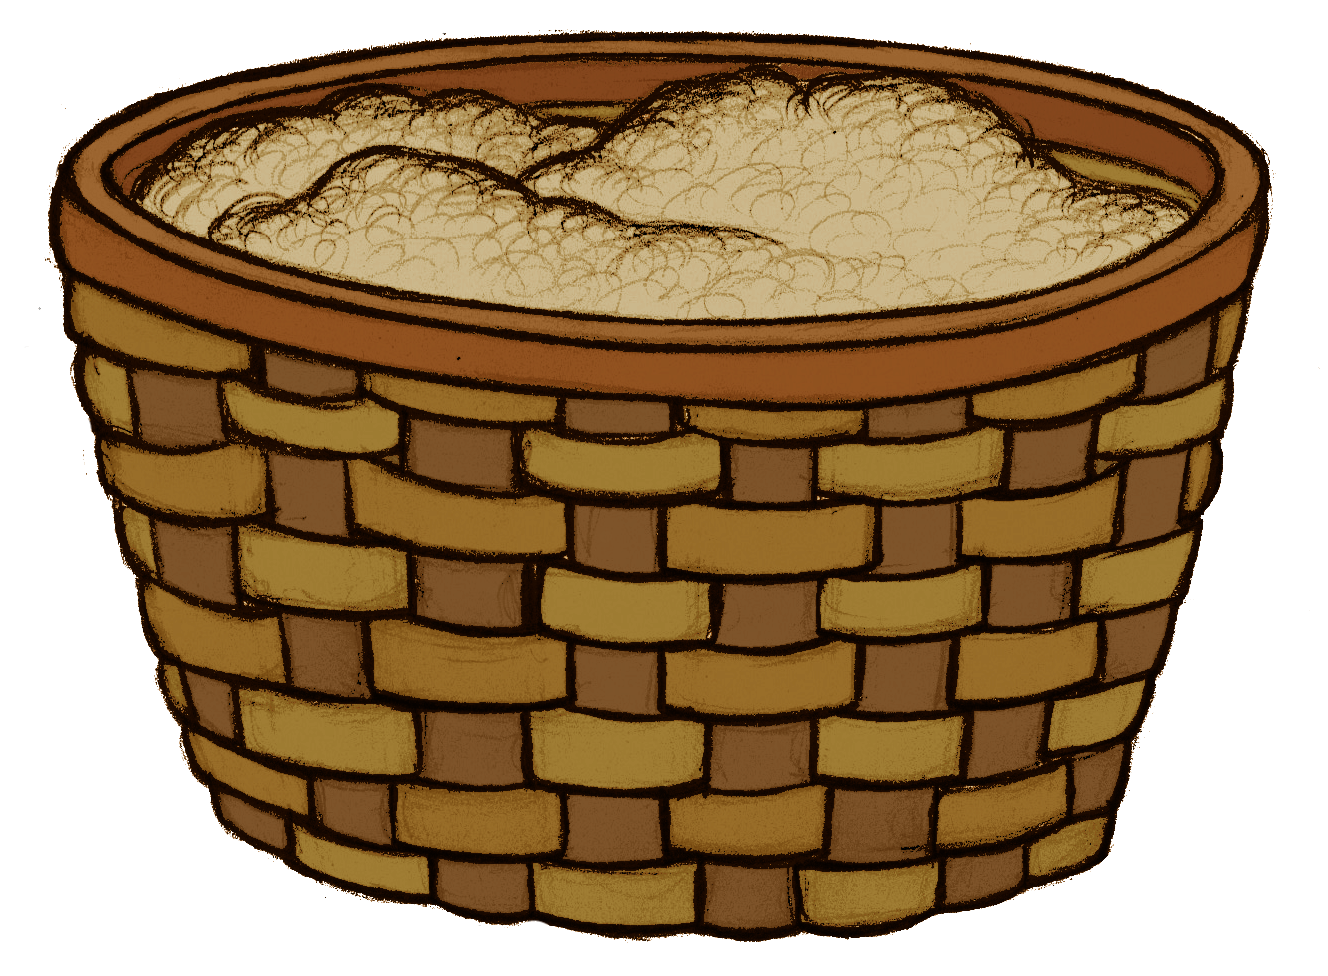
\includegraphics[height=30mm]{img/Jorvik/objects/weaver/raw wool}}\\
		\DIFaddFL{Raw Wool }& \\ 
		\textbf{\DIFaddFL{Price:}} & \\
		\DIFaddFL{1.32 Silver. }& \\ 
		\textbf{\DIFaddFL{Description:}} & \\
		\multicolumn{2}{p{12cm}}{Wool would be used for making most of the Viking Age fabric. It was used to make tunics, trousers, dresses, socks, cloaks and hangeroks (aprons).}\\
		\bottomrule
	\end{tabular}
\end{table}

\begin{table}[ht!]
	\centering
	\begin{tabular}{ p{3cm} c }\toprule
		\textbf{\DIFaddFL{Name:}} & \multirow{5}{*}{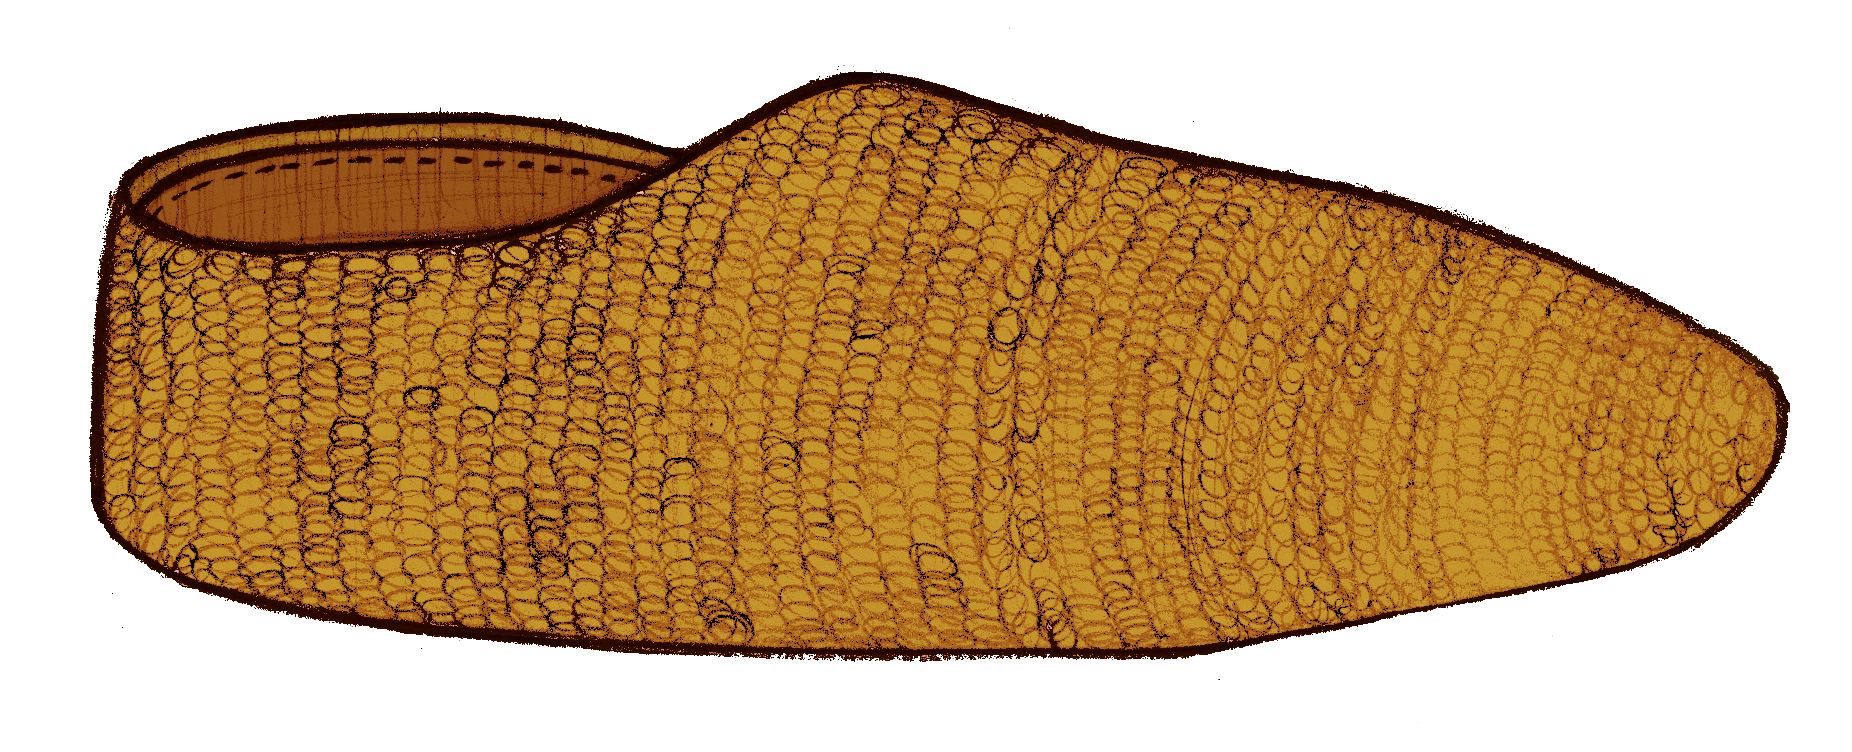
\includegraphics[width=70mm]{img/Jorvik/objects/weaver/socks}}\\
		\DIFaddFL{Socks }& \\ 
		\textbf{\DIFaddFL{Price:}} & \\
		\DIFaddFL{4.41 Silver. }& \\ 
		\textbf{\DIFaddFL{Description:}} & \\
		\multicolumn{2}{p{12cm}}{Socks were for the wealthiest Vikings. Those who could not afford socks might have lined their shoes with moss, grasses, or un-spun wool.}\\
		\bottomrule
	\end{tabular}
\end{table}

\begin{table}[ht!]
	\centering
	\begin{tabular}{ p{3cm} c }\toprule
		\textbf{\DIFaddFL{Name:}} & \multirow{5}{*}{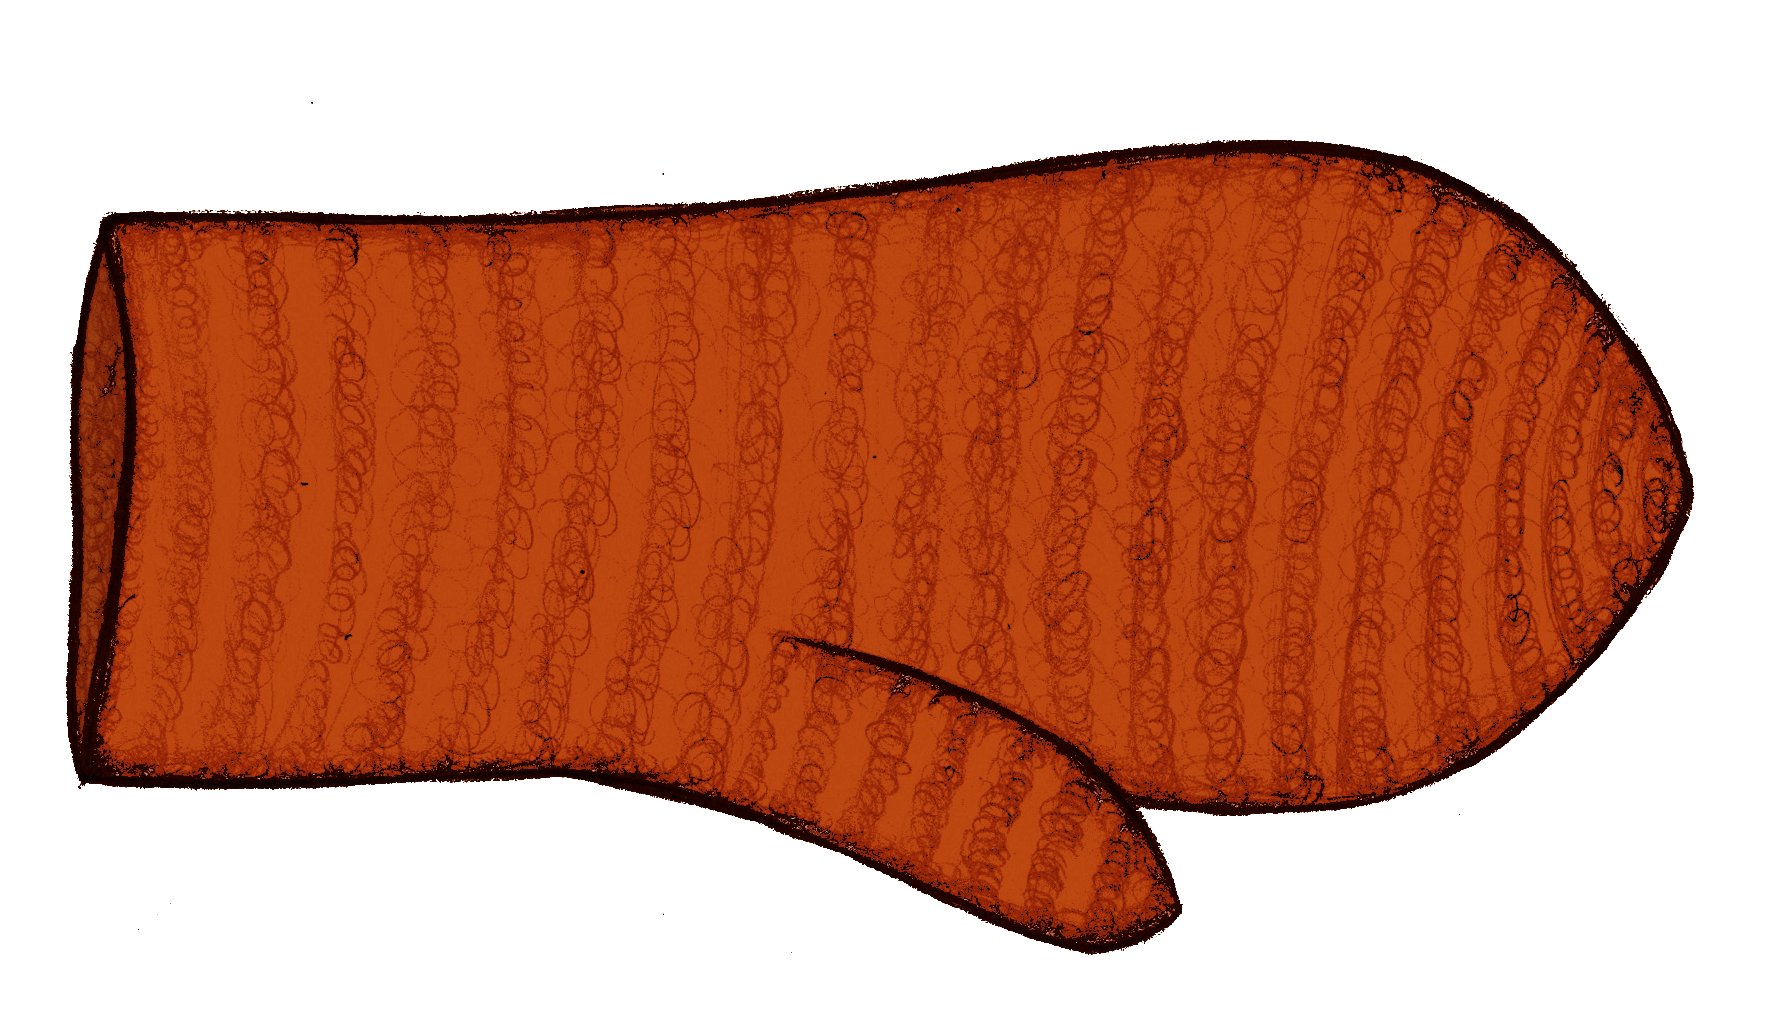
\includegraphics[height=30mm]{img/Jorvik/objects/weaver/mittens}}\\
		\DIFaddFL{Mittens }& \\ 
		\textbf{\DIFaddFL{Price:}} & \\
		\DIFaddFL{3.97 Silver. }& \\ 
		\textbf{\DIFaddFL{Description:}} & \\
		\multicolumn{2}{p{12cm}}{Mittens could be made using naalbinding techniques with a single needle or by simply sewing together two pieces of fabric.}\\
		\bottomrule
	\end{tabular}
\end{table}

\begin{table}[ht!]
	\centering
	\begin{tabular}{ p{3cm} c }\toprule
		\textbf{\DIFaddFL{Name:}} & \multirow{5}{*}{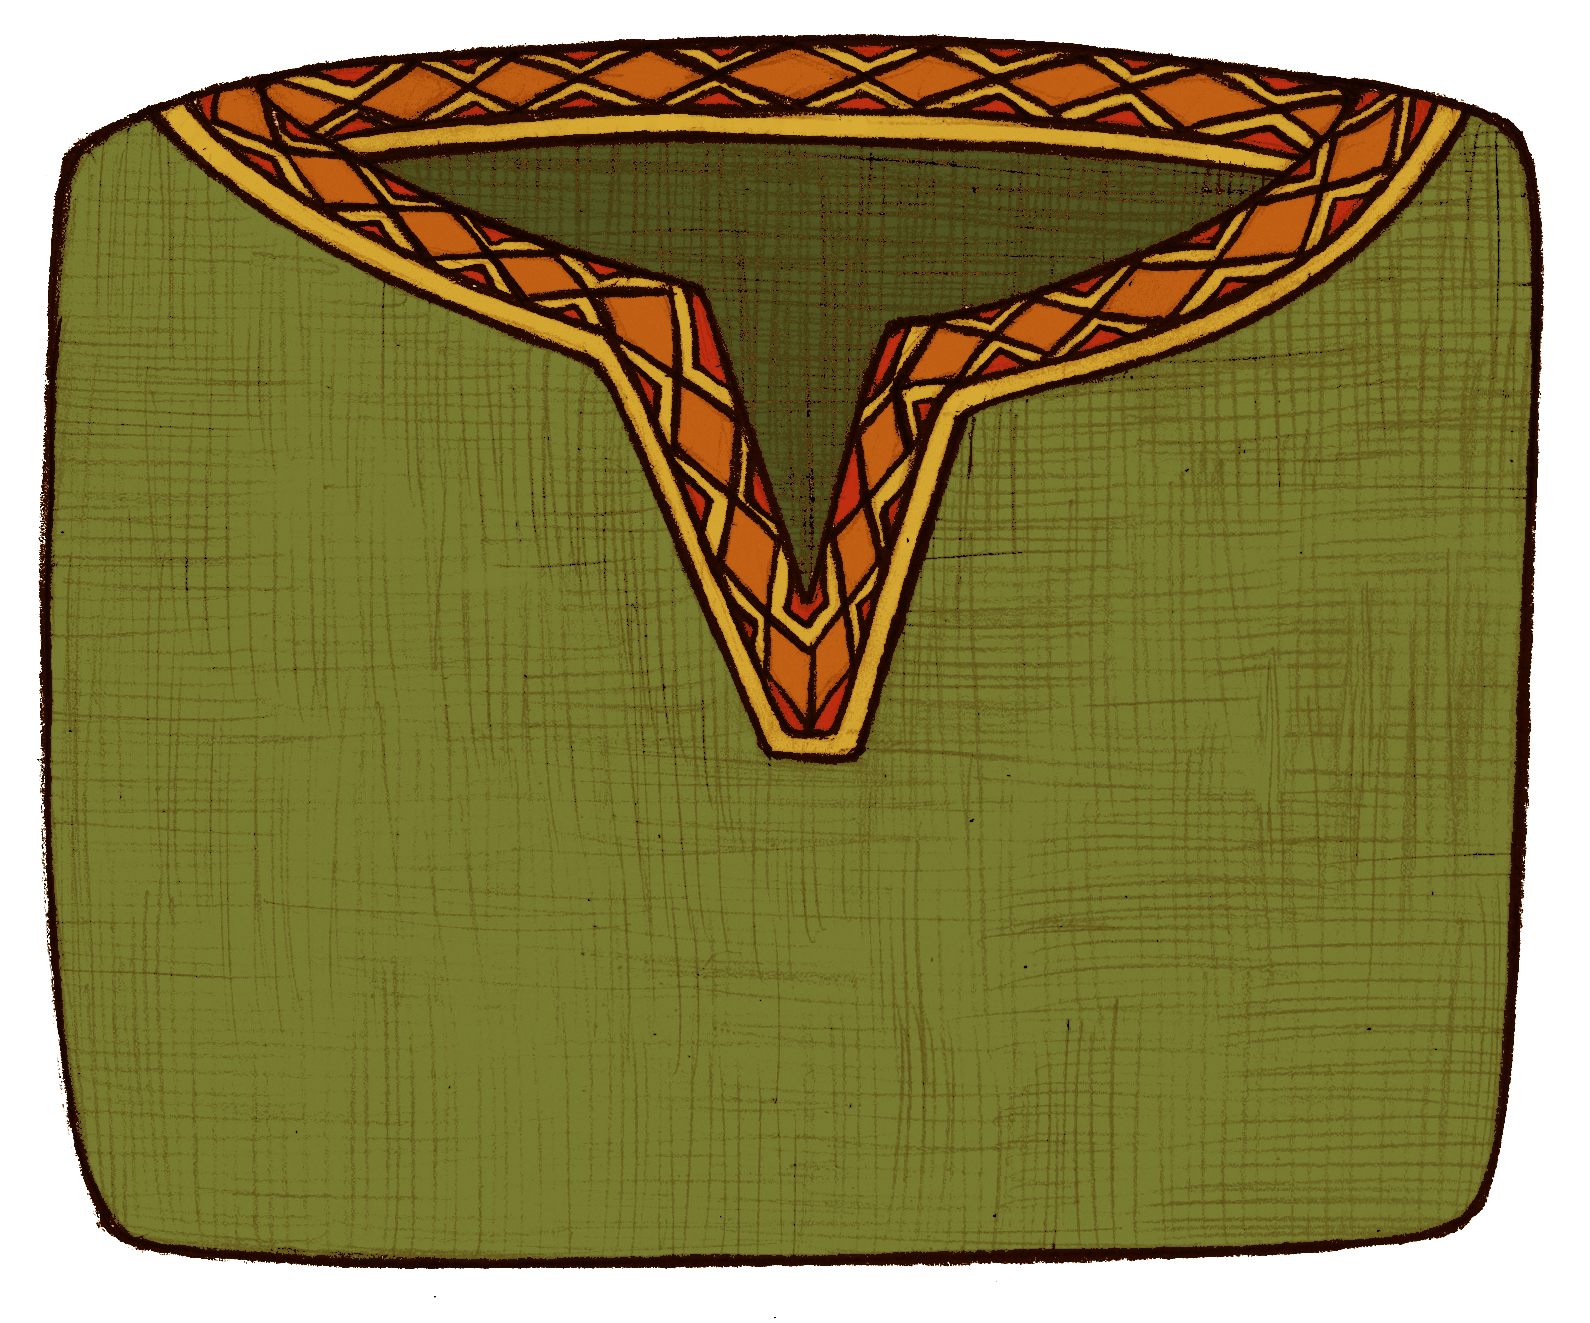
\includegraphics[height=30mm]{img/Jorvik/objects/weaver/tunic}}\\
		\DIFaddFL{Tunic }& \\ 
		\textbf{\DIFaddFL{Price:}} & \\
		\DIFaddFL{5.29 Silver. }& \\ 
		\textbf{\DIFaddFL{Description:}} & \\
		\multicolumn{2}{p{12cm}}{Vikings wore simple tunics that rarely had fasteners. Men's necklines were high because a wife could divorce her husband if he showed too much of his chest! Likewise, a man could divorce his wife for wearing trousers!}\\
		\bottomrule
	\end{tabular}
\end{table}

\begin{table}[ht!]
	\centering
	\begin{tabular}{ p{3cm} c }\toprule
		\textbf{\DIFaddFL{Name:}} & \multirow{5}{*}{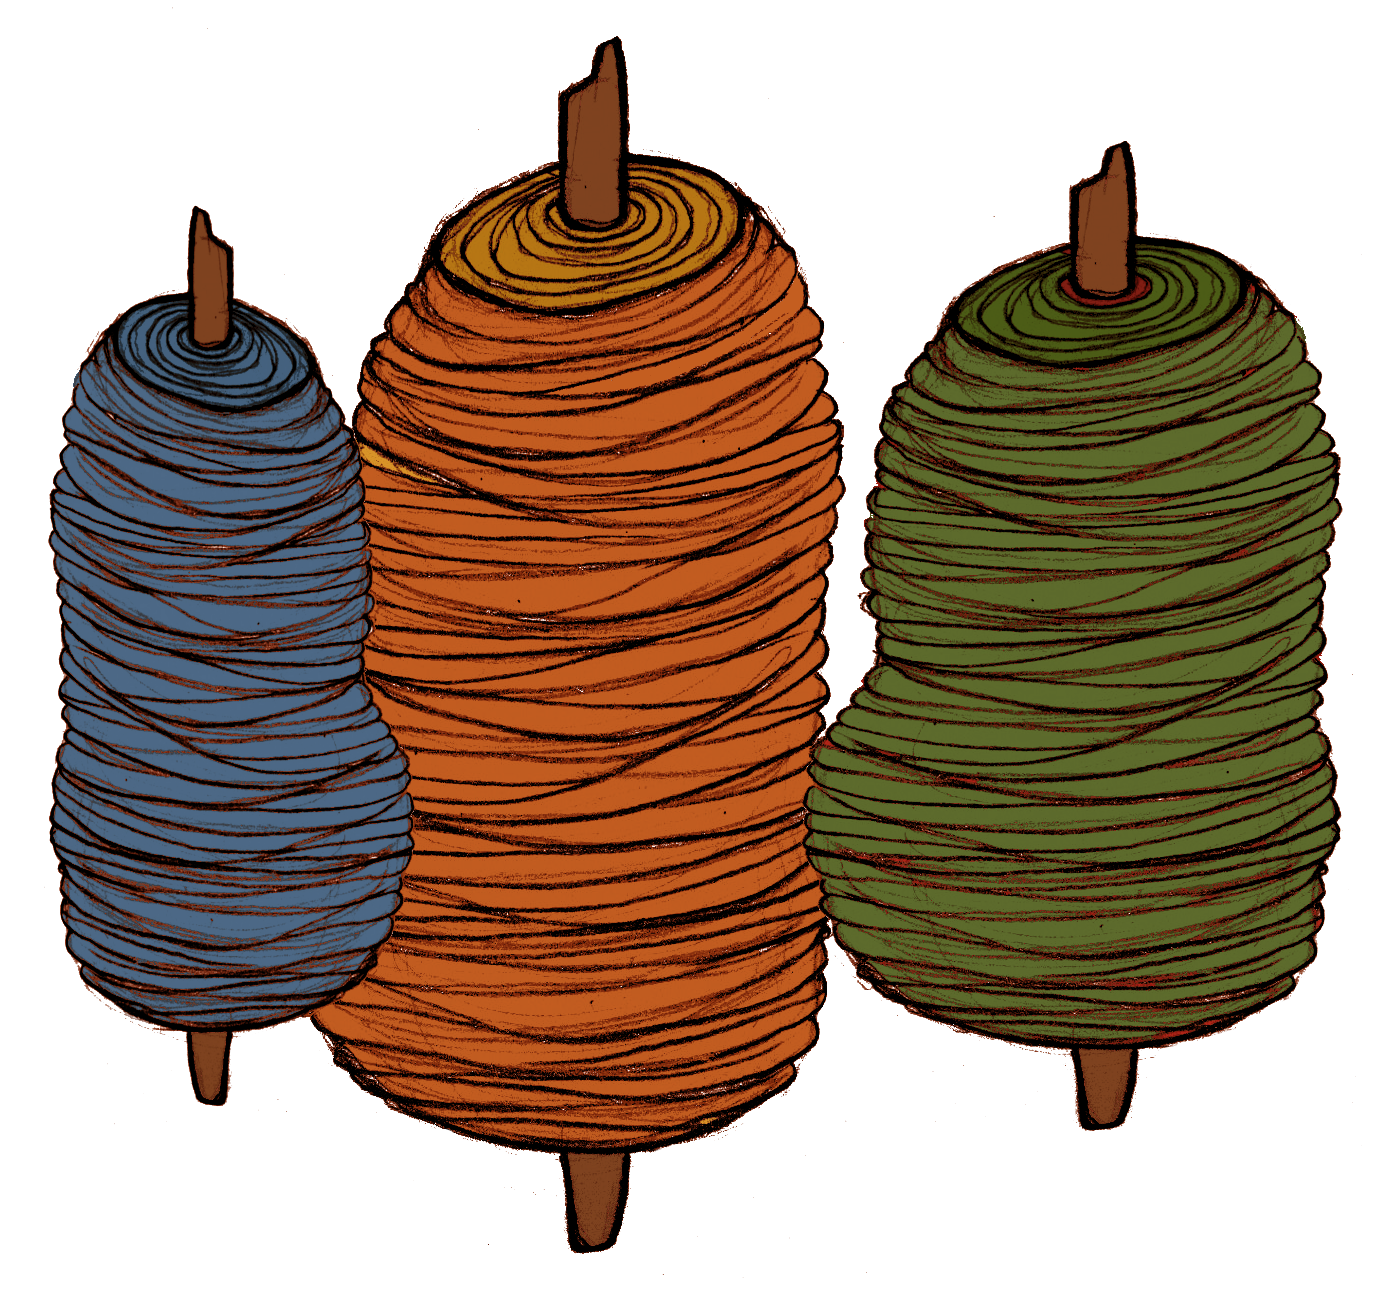
\includegraphics[height=30mm]{img/Jorvik/objects/weaver/yarn}}\\
		\DIFaddFL{Yarn }& \\ 
		\textbf{\DIFaddFL{Price:}} & \\
		\DIFaddFL{2.21 Silver. }& \\ 
		\textbf{\DIFaddFL{Description:}} & \\
		\multicolumn{2}{p{12cm}}{The process of making clothes was a long one. First the wool was spun into yarn, then it was dyed, then it was woven into cloth and finally it was cut and sewn into clothes. The process would take several days.}\\
		\bottomrule
	\end{tabular}
\end{table}

\begin{table}[ht!]
	\centering
	\begin{tabular}{ p{3cm} c }\toprule
		\textbf{\DIFaddFL{Name:}} & \multirow{5}{*}{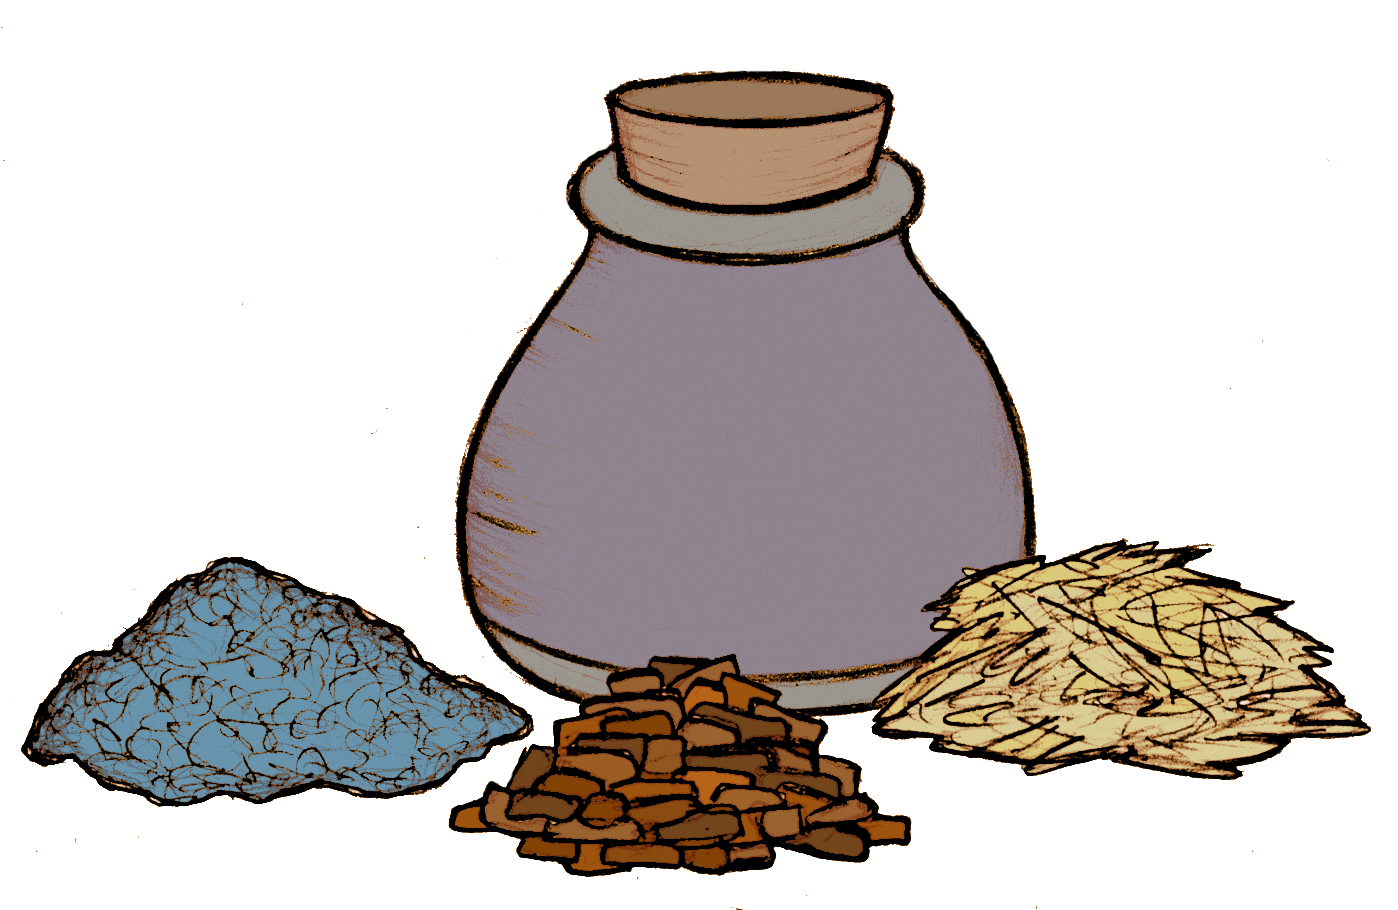
\includegraphics[height=30mm]{img/Jorvik/objects/weaver/dye}}\\
		\DIFaddFL{Dye }& \\ 
		\textbf{\DIFaddFL{Price:}} & \\
		\DIFaddFL{4,41 Silver. }& \\ 
		\textbf{\DIFaddFL{Description:}} & \\
		\multicolumn{2}{p{12cm}}{The Vikings used plants to make different dyes to colour their clothes. They got red from madder, yellow from weld, blue from woad, and orange from onion skins!}\\
		\bottomrule
	\end{tabular}
\end{table}

\begin{table}[ht!]
	\centering
	\begin{tabular}{ p{3cm} c }\toprule
		\textbf{\DIFaddFL{Name:}} & \multirow{5}{*}{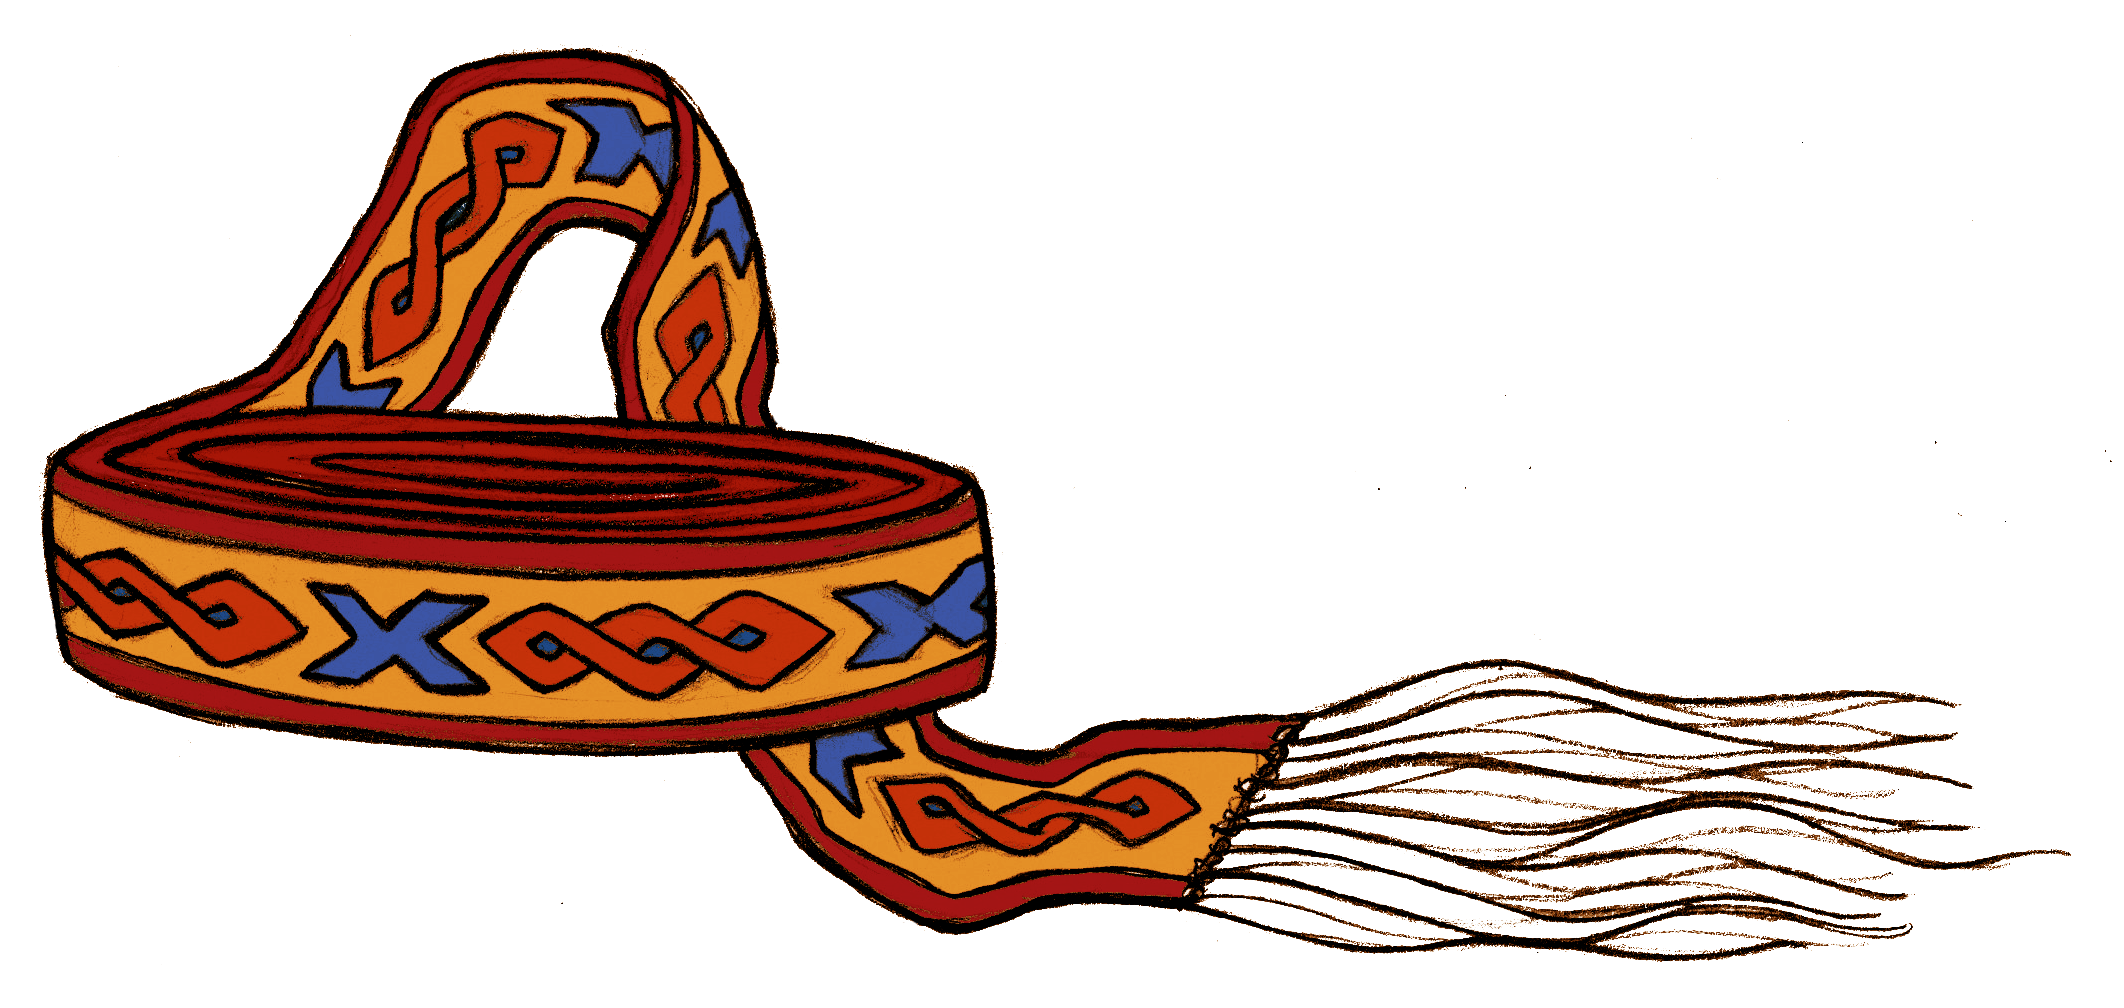
\includegraphics[height=30mm]{img/Jorvik/objects/weaver/braid}}\\
		\DIFaddFL{Braid }& \\ 
		\textbf{\DIFaddFL{Price:}} & \\
		\DIFaddFL{3.97 Silver. }& \\ 
		\textbf{\DIFaddFL{Description:}} & \\
		\multicolumn{2}{p{12cm}}{Braids were made through a process called tablet weaving. Braids would be used to line cloaks and tunics to make them more decorative. Tablet weaving was a long process so were very expensive.}\\
		\bottomrule
	\end{tabular}
\end{table} \DIFaddend